\chapter{Robots and controllers evaluated}
\label{chap:robots}
In this chapter, we describe the experiments conducted to validate our approach. Since this thesis is focused on using simulation to speed up hardware experiments, robot experiments form an important part of this work. Our hardware experiments are done on the ATRIAS robot on a boom to make the robot planar to two dimensions. It is mounted on a pivot, so it can still fall down. We present results on a feedback based reactively stepping controller, optimizing 5 and 9 parameters in 2 sets of experiments on hardware. 

Our simulation experiments are conducted on two different robot morphologies -- a planar 7-link biped model, and an ATRIAS simulation on the boom. We present two neuromuscular walking controllers -- on a 7-link biped optimizing 16 parameters, and then on an ATRIAS simulation optimizing 50 parameters.

In addition, we present experiments on learning neural network policies using deep reinforcement learning. These policies are learned in simulation and deployed on the ATRIAS biped.

We detail our robots in the next section, followed by the controllers. 

\section{Robot morphologies tested}

\subsection{The ATRIAS Robot}
\label{sec:atrias}
Our test platform is CMU's ATRIAS robot (Figure \ref{fig:atrias}), a human sized bipedal robot \citep{hubicki2016atrias}. The ATRIAS robot was designed so that the inertial properties of the center of mass of ATRIAS matched that of humans. The robot weights about $64kg$, with most of its mass concentrated around the trunk. The torso is located about $0.19m$ above the pelvis, and its rotational inertia is about $2.2 kgm^2$. The legs are 4-segment carbon-fiber linkages driven with a point foot, making the legs very light and enabling fast swing movements. The legs are actuated by 2 Series Elastic Actuators (SEAs) in the sagittal plane and a DC motor in the lateral plane. The SEAs consist of a fiberglass leaf spring attached to a geared DC motor on one end and the leg load on the other. Each spring is equipped with a load-side and motor-side encoder, which given the spring stiffness, can be used to estimate joint torques on each joint. 
Although ATRIAS is capable of 3D walking, in this work, we focus on planar movements around a boom.
%The rotational variables of the Center of Mass, such as the pitch, roll, etc. are measured through sensors attached on the boom.

\subsection{A 7-link biped model}
\label{sec:7_link_biped}
%\begin{figure}[t]
%    \centering
%    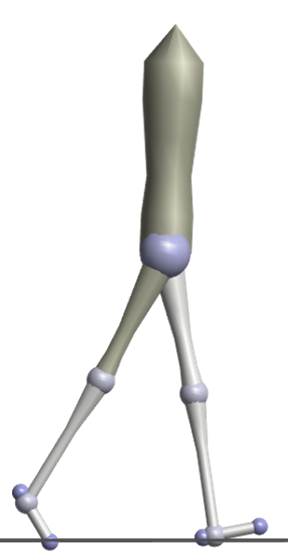
\includegraphics[height=0.3\textheight]{img/7link.png}
%    \caption{The 7-link planar biped model}
%    \label{fig:planar_biped}
%\end{figure}
We also experiment with a 7-link planar 2-dimensional human-like robot model as shown in Figure \ref{fig_nmm}. It has two legs - composed of foot, shin and thigh and a hip. There are 6 actuators at the ankle, knee and hip joints in each leg with infinite allowed torque. This model is used as a simple 2-dimensional approximation to more complex humanoid robots. 

\section{Controllers tested}

\subsection{Neuromuscular model for humanoid robots}

\label{sec:NMC}
We use neuromuscular model policies, as introduced in \cite{geyer2010muscle}, as our controller for a 7-link planar human-like model. These policies use approximate models of muscle dynamics and human-inspired reflex pathways to generate joint torques, producing gaits that are similar to human walking in stance. \cite{desai} designed reflex laws for swing that enable target foot-placement and leg clearance, by analyzing the double pendulum dynamics of the human leg. Integrating this swing control with the previous reflex control enables the model to overcome disturbances in the range of up to $\pm 10 cm$, as described in \cite{song2015neural}. We next describe this control in some detail.

\subsubsection{Neuromuscular Stance Control} 

In stance of the neuromuscular controller, each leg is actuated by 7 Hill-type muscles \cite{morrison1970mechanics}, consisting of the soleus (SOL), gastrocnemius (GAS), vastus (VAS), hamstring (HAM), tibialis anterior (TA), hip flexors (HFL) and gluteus (GLU), illustrated in Figure \ref{fig_nmm}. Together, these muscles produce torques about the hip, knee and ankle. The muscle force $F$ is a non-linear function of the muscle state $s^m$ and stimulus $S^m$, which when multiplied by the moment arm $r(\theta_i)$ gives the resultant torque on joint $i$:
\begin{equation*}
\tau_i^m = F(S^m, s^m)r(\theta_i),
\end{equation*}   
where $\tau_i^m$ is the torque applied by muscle $m$ on joint $i$ and $\theta_i$ is the joint angle.
 
\begin{figure}[t]
    \centering
    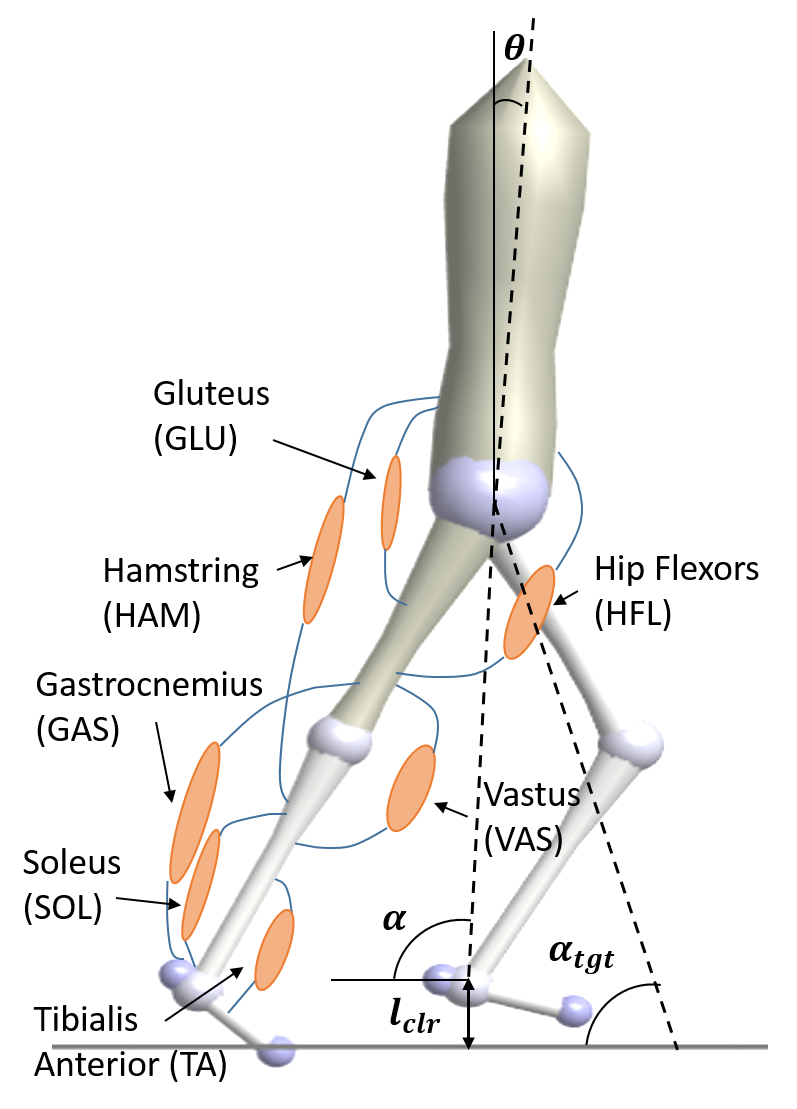
\includegraphics[height=0.3\textheight]{img/nmm_pic.png}
    \caption{The neuromuscular model. The muscles and swing parameters are highlighted.}
    \label{fig_nmm}
\end{figure}

Most of the muscle reflexes in stance are positive length or force feedback on the muscle stimulus. In general, the stimulus $S^m(t)$ for muscle $m$ is a function of the time delayed length or force signal $P^m$ times a feedback gain $K^m$:
\begin{equation*}
S^m(t) =  S_0^m + K^m \cdot P^m(t - \Delta t),
\end{equation*}
where $S_0^m$ is the pre-stimulus, $K^m$ is the feedback gain and $P^m$ is the time-delayed feedback signal of length or force. Some muscles can be co-activated and have multiple feedback signals from more than one muscle. The feedback gains $K^m$ described above are a subset of the parameters that we aim to tune in our optimization. The details of these feedback pathways can be found in \cite{song2015neural}.

This feedback structure generates compliant leg behaviour and prevents the knee from overextending in stance. To balance the trunk, feedback on the torso angle is added to the GLU stimulus:
\begin{equation*}
S^{GLU}_{torso}(t) = K_p^{stance}(\theta_{des} - \theta) -K_d^{stance}\dot{\theta},
\end{equation*}
where $K_p^{stance}$ is the position gain on the torso angle $\theta$ and $\theta_{des}$ is the desired angle. $K_d^{stance}$ is the velocity gain and $\dot{\theta}$ is the angular velocity.
Specifically, here are the stance parameters we optimize over, and their roles in the neuromuscular model:
 
\begin{itemize}
\item $K^{GAS}$ : Positive force feedback gain on GAS
\vspace{-2mm}
\item $K^{GLU}$ : Positive force feedback gain on GLU
\vspace{-2mm}
\item $K^{HAM}$ : Positive force feedback gain on HAM
\vspace{-2mm}
\item $K^{SOL}$ : Positive force feedback gain on SOL
\vspace{-2mm}
\item $K^{TA}_{SOL}$ : Negative force feedback from SOL on TA
\vspace{-2mm}
\item $K^{TA}$ : Positive length feedback on TA
\vspace{-2mm}
\item $K^{VAS}$ : Positive force feedback on VAS
\vspace{-2mm}
\item $K^{stance}_p$ : Position gain on feedback on torso angle
\vspace{-2mm}
\item $K^{stance}_d$ : Velocity gain on feedback on torso velocity
\vspace{-2mm}
\item $K_{mix}^{GLU}$ : Gain for mixing force feedback and feedback on angle for GLU
\end{itemize}

\subsubsection{Swing Leg Placement Control}

The swing control is controlled by three main components -- target leg angle, leg clearance and hip control. Target leg angle is a direct result of the foot placement strategy which is a function of the velocity of the center of mass (CoM) $v$, and the as distance between the stance leg the CoM, and presented in \cite{simbicon}:
\begin{equation*}
\alpha_{tgt} = \alpha_0 + C_d d + C_v v,
\end{equation*}
where $\alpha_{tgt}$ is the target leg angle, $\alpha_0$ is the nominal leg angle, $\alpha_0$, $C_d$ and $C_v$ are parameters optimized by our control.

Leg clearance is a function of the desired leg retraction during swing. The knee is actively flexed until the leg reaches the desired leg clearance height, $l_{clr}$ and then held at this height, until the leg reaches a threshold leg angle. At this point, the knee is extended and allowed to reach the target leg angle $\alpha_{tgt}$. Details of this control can be found in \cite{desai}. As was noted in \cite{song2015neural}, and observed in our experiments, the control is relatively insensitive to the individual gains of the set-up in swing. It is sufficient to control the higher level parameters such as the desired leg clearance and target leg angle.

The third part of the control involves maintaining the desired leg angle $\alpha_{tgt}$ by applying a hip torque $\tau_{hip}^{\alpha}$:
\begin{equation*}
\tau_{hip}^{\alpha} = K_p^{swing}(\alpha_{tgt} - \alpha) - K_d^{swing}(\dot{\alpha}),
\end{equation*}
where $K_p^{swing}$ is the position gain on the leg angle, $K_d^{swing}$ is the velocity gain, $\alpha$ is the leg angle and $\dot{\alpha}$ is the leg angular velocity (see Figure \ref{fig_nmm}). 

More concisely, the swing parameters that we focus on in our optimization are the following:
\begin{enumerate}
\item $K_p^{swing}$ : Position gain on feedback on leg angle
\vspace{-2mm}
\item $K_d^{swing}$ : Velocity gain on feedback on leg velocity
\vspace{-2mm}
\item $\alpha_0$ : Nominal leg angle
\vspace{-2mm}
\item $C_d$ : Gain on the horizontal distance between the stance foot and CoM
\vspace{-2mm}
\item $C_v$ : Gain on the horizontal velocity of the CoM
\vspace{-2mm}
\item $l_{clr}$ : Desired leg clearance
\end{enumerate}

Though originally developed for explaining human neural control pathways, these controllers have recently been applied to robots and prosthetics, for example in \cite{thatte} and \cite{van2015biped}. As demonstrated in \cite{song2015neural}, these models are indeed capable of generating a variety of locomotion behaviours for a humanoid model - for example, walking on flat, rough ground, turning, running, walking upstairs and on ramps. However, a full study of using these models to control biped robots still needs to be done. Whether these models will transfer well to robots with significantly different dynamics and inertial properties than humans needs to be explored. It is difficult to transfer these models to robots because of a large number of interdependent gains that need to be tuned. Typically, this is done using Covariance Matrix Adaptation Evolutionary Strategy \mbox{(CMA-ES)} \citep{hansen2006cma}, an evolutionary algorithm for difficult non-linear non-convex black-box optimization problems. Even though CMA-ES is useful for optimizing non-convex problems in high dimensions, it is not sample efficient and depends on the initial starting point. An optimization for 16 neuromuscular parameters takes 400 generations, around a day on a standard i7 processor and about 5,000 trials, as reported in \cite{song2015neural}. 

The large number of trials make it impossible to implement CMA-ES on a real robot. This is a shortcoming because often we find that after training the policies in simulation, they do not transfer well to the real robot, due to differences between simulation and real hardware. We aim to overcome this problem by using Bayesian Optimization with informed feature transforms for optimizing controllers.
%In the following sections, we will develop a sample efficient method for training the same controller. 

The neuromuscular controller is a model-free controller. It does not need the exact dynamics of the robot to generate torques. The dynamics are inherently embedded in the learned parameters of the controller. As a result, the same controller can be used on very different robots without any modification to the policy structure. 

We next describe a model-based reactively stepping controller. This controller uses the dynamics models of the robot to generate torques. Hence, to transfer to new systems, the dynamics need to be updated.


\subsection{Feedback based reactive stepping policy}
\label{sec:raibert_cont}
We design a parametric controller for controlling the CoM height, torso angle and the swing leg by commanding desired ground reaction forces and swing foot landing location. 
\begin{align}
    \label{eq:raibert}
    F_x = K_{pt}(\theta_{des} - \theta) + K_{dt}(\dot{\theta}_{des} - \dot{\theta}) \\
    F_z = K_{pz}(z_{des} - z) + K_{dz}(\dot{z}_{des} - \dot{z})\\
    x_p = k(v-v_{tgt}) + C \cdot d + 0.5 \cdot v \cdot T
\end{align}
Here, $F_x$ is the desired horizontal ground reaction force (GRF), $K_{pt}$ is the proportional gain on the torso angle $\theta$ and $K_{dt}$ is the derivative gain on the torso angular velocity $\dot{\theta}$. $\theta_{des}$ and $\dot{\theta}_{des}$ are the desired torso lean and desired torso angular velocity. $F_z$ is the desired vertical GRF, $K_{pz}$ is the proportional gain on the CoM height $z$ and $K_{dz}$ is the derivative gain on the CoM vertical velocity $\dot{z}$. $z_{des}$ and $\dot{z}_{des}$ are the desired CoM height and desired CoM vertical velocity. Both $\dot{\theta}_{des}$ and $\dot{z}_{des}$ are always set to $0$. $x_p$ is the desired foot landing location for the end of swing; $v$ is the horizontal CoM velocity, $k$ is the feedback gain that regulates $v$ towards the target velocity $v_{tgt}$. These quantities are highlighed in Figure \ref{fig:raibert_com}. $C$ is a constant and $d$ is the distance between the stance leg and the CoM; $T$ is the swing time and the term $0.5 \cdot v \cdot T$ is a feedforward term similar to a Raibert hopping policy, described in \cite{raibert1986legged}.
\begin{figure}[t]
    \centering
    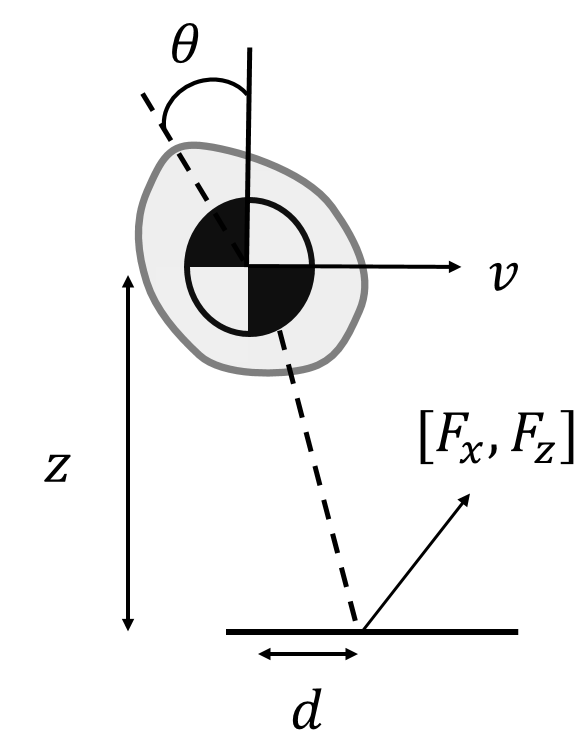
\includegraphics[width=0.3\textwidth]{img/raibert_com.png}
    \caption{\small{Illustration of the Center of Mass model and variables used for the feedback-based stepping policy.}}
    \label{fig:raibert_com}
\end{figure}

This parametrization results in desired ground reaction forces (GRFs) in stance and a desired foot landing position in swing. Note that there is no desired CoM trajectory in this controller. We only command a desired CoM velocity, regulated through the swing foot placement. In stance, the desired GRFs regulate a desired CoM height and torso angle. These are then sent to the ATRIAS inverse dynamics model that generates desired motor torques $(\tau_f, \tau_b)$ that realize the GRFs. 
\begin{equation}
    M \ddot{q} + h = S \tau + J^T F
\end{equation}
where $M$ is the mass matrix, $\ddot{q}$ are the joint accelerations, $h$ are the gravitational terms, $S$ is a selection matrix, $\tau$ are resultant joint torques, $J$ is the contact Jacobian and $F = [F_x, F_z]$ are the desired forces generated in \ref{eq:raibert}. There are no Coriolis terms due to the assumption of massless legs. Details can be found in \cite{wu2014highly}. These desired motor torques are then sent to a low level motor velocity-based feedback loop that generates the desired torques in the robot SEAs. % (Fig \ref{fig:control_flow}). 

In swing, we continually re-generate a 5th order spline that starts from the current position and velocity of the swing leg, $x_{sw}$ and $\dot{x}_{sw}$ and terminates at the desired foot position $x_{fp}$, with ground speed matching (swing leg is at rest with respect to the ground). The desired initial and final point of this spline is continually regenerated based on the current estimate of the swing foot position and velocity, as well as the desired footstep and CoM velocity. This trajectory gives the next desired position and velocity of the swing leg, $x_{sw}^*$, $\dot{x}_{sw}^*$, which is translated to desired joint positions and velocities using the robot kinematics. These are then position-controlled by sending a velocity command to the robot SEAs. % (Fig \ref{fig:control_flow}).

%\begin{figure}[t]
%    \centering
%    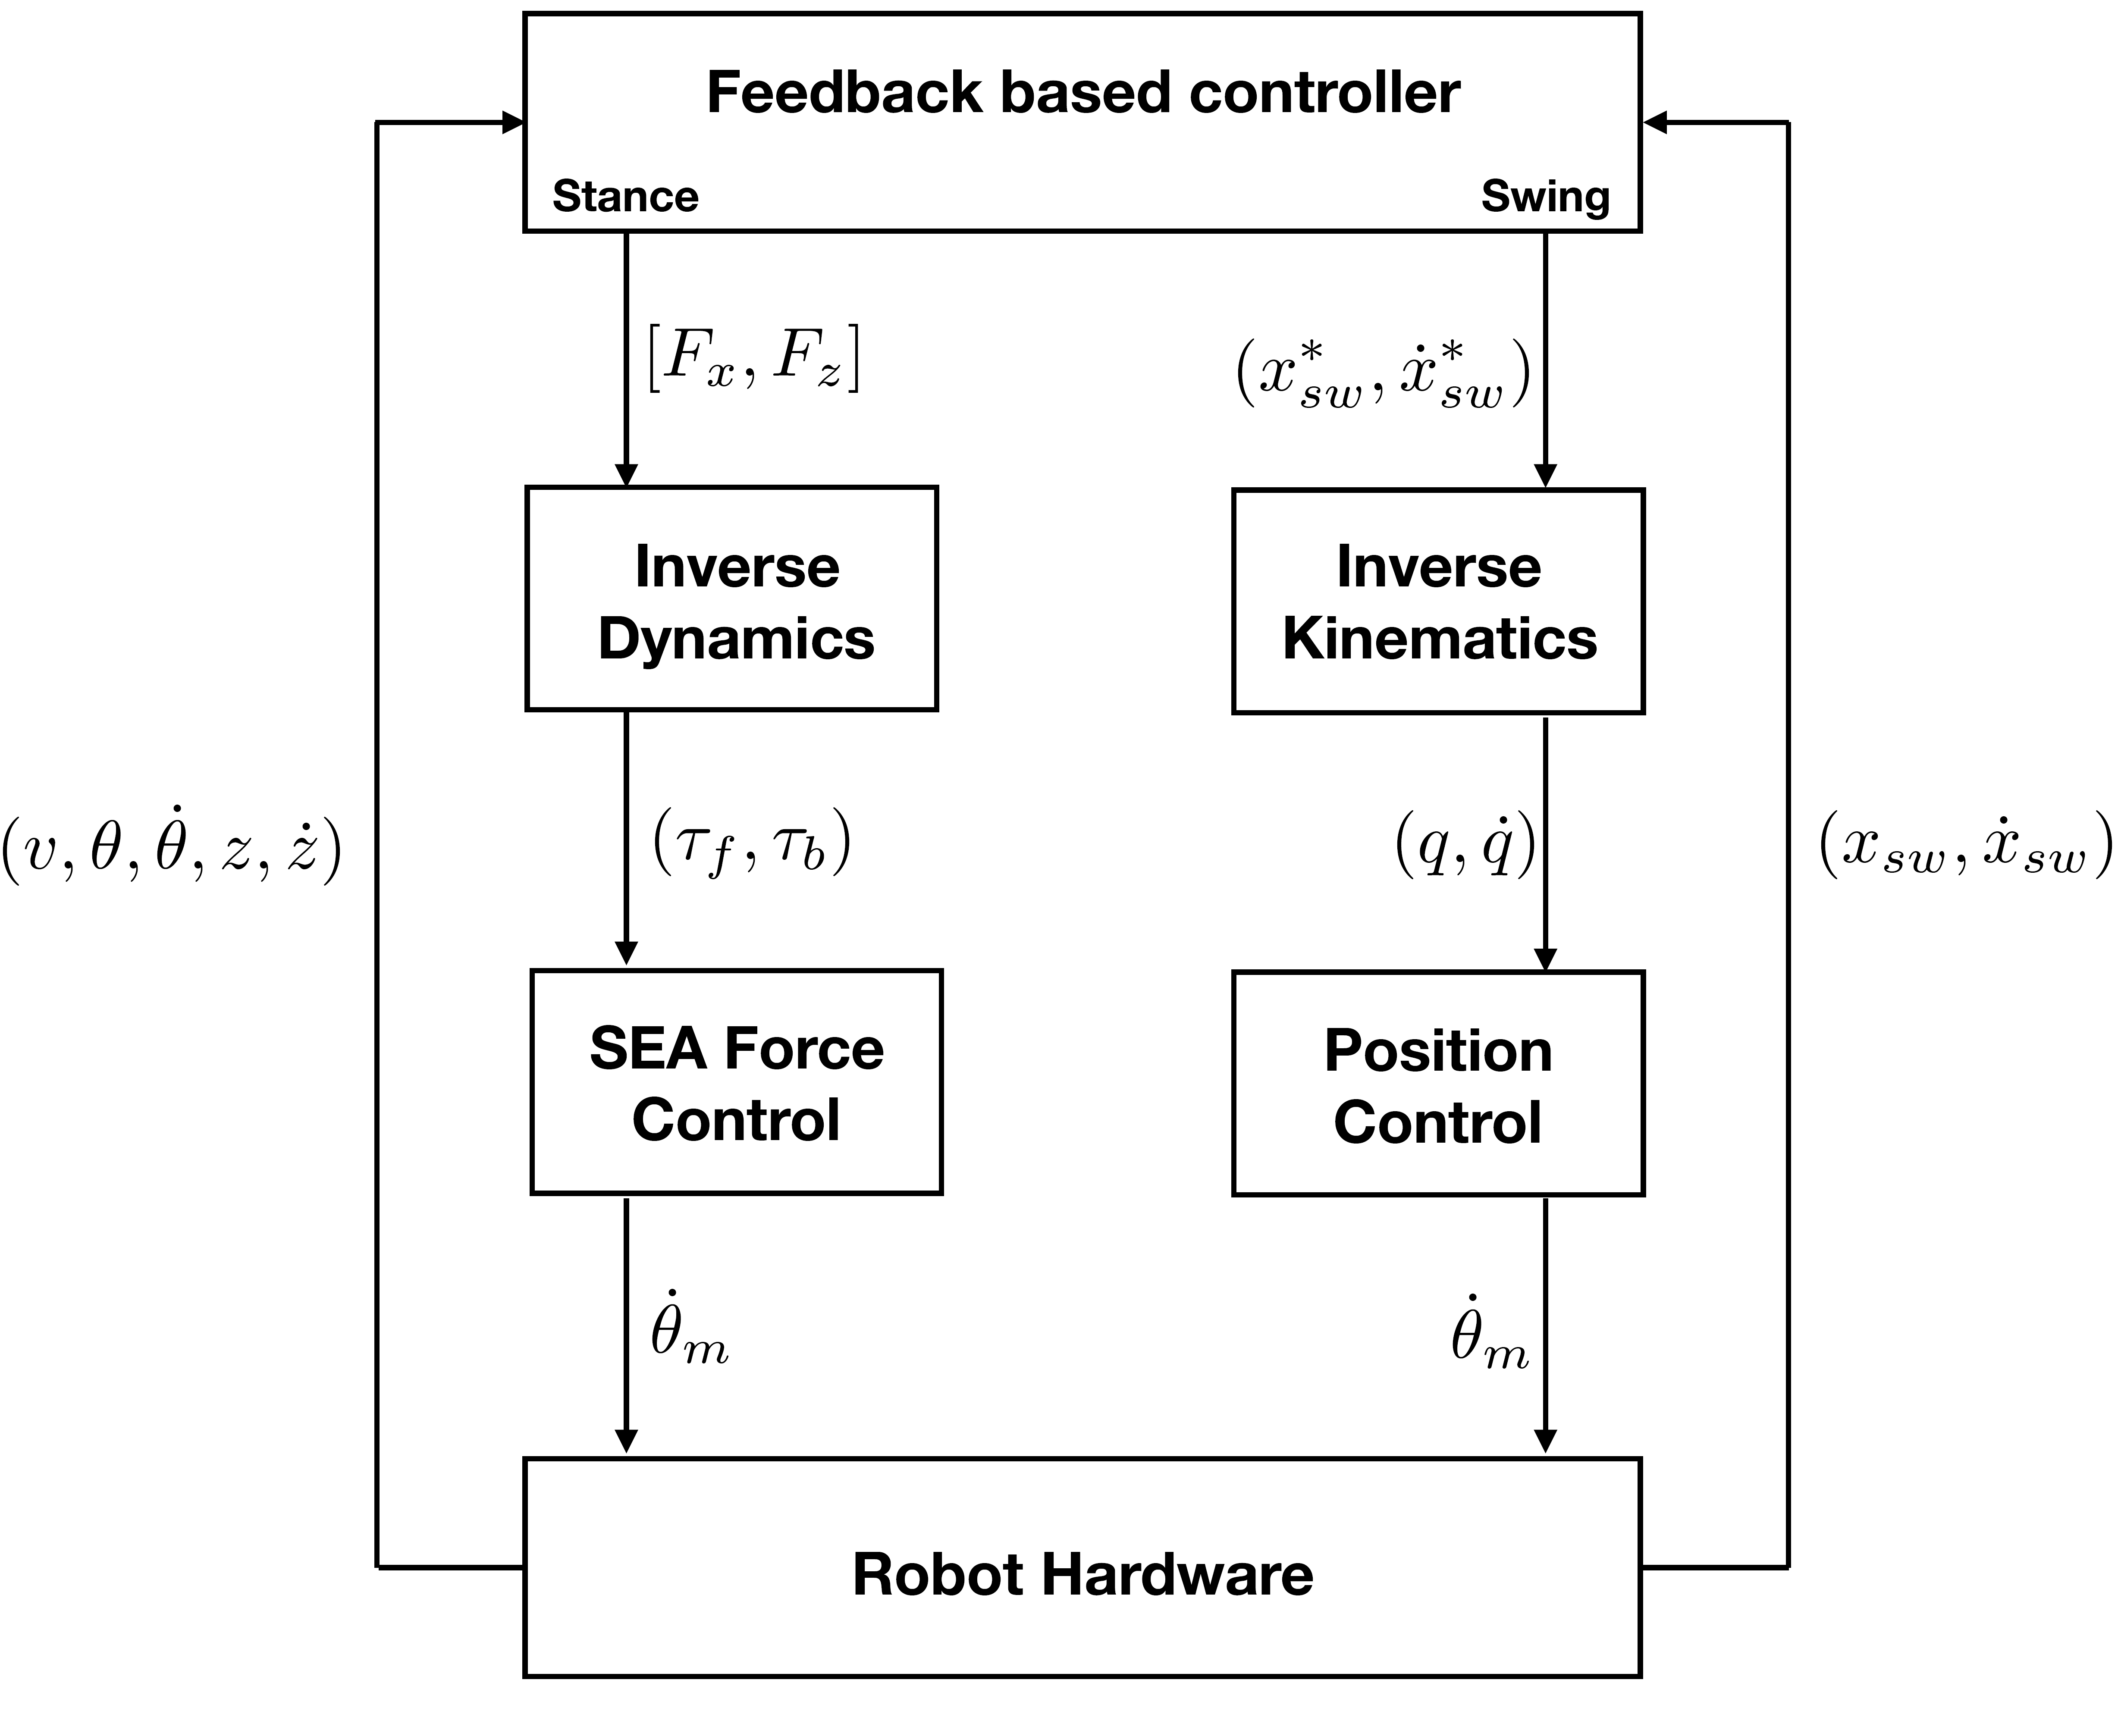
\includegraphics[width=0.8\textwidth]{img/flowchart_cropped.png}
%    \caption{\small{ATRIAS control flowchart with variables from Section~\ref{sec:raibert_cont}}}
%    \label{fig:control_flow}
%\end{figure}

This controller assumes no double-stance, the swing leg takes off as soon as stance is detected. This leads to a highly dynamic gait, as the contact polygon for ATRIAS in single stance is a point. It should be possible to extend this walking controller to include a double stance phase, but we leave that to future work. 

The controller also depends on the desired speed of walking (as this determines the next stepping location). This means that the ``stability" of the controller depends not only on the parameters chosen, but also the desired target speed. We assume that the target speed is provided by the user and is constant in our experiments. It is possible to add the desired speed as an extra dimension to the controller and optimize controllers conditioned on this. But we leave that for future work.

\begin{enumerate}
    \item 5 dimensional walking controller : In our first set of experiments, we optimized 5 parameters from the above described controller. These were $[K_{pt}, K_{dt}, k, C, T]$. The desired positions and velocities were hand tuned, and so was the feedback on $z$.
    \item 9 dimensional walking controller : In our second set of experiments, we optimized 9 parameters of the above described controller. They were :
    
    $[K_{pt}, K_{dt}, \theta_{des}, K_{pz}, K_{dz}, z_{des}, k, C, T]$
\end{enumerate}

\subsection{Virtual Neuromuscular Controller for ATRIAS}
\label{sec:VNMC_cont}

\begin{figure}[t]
\centering
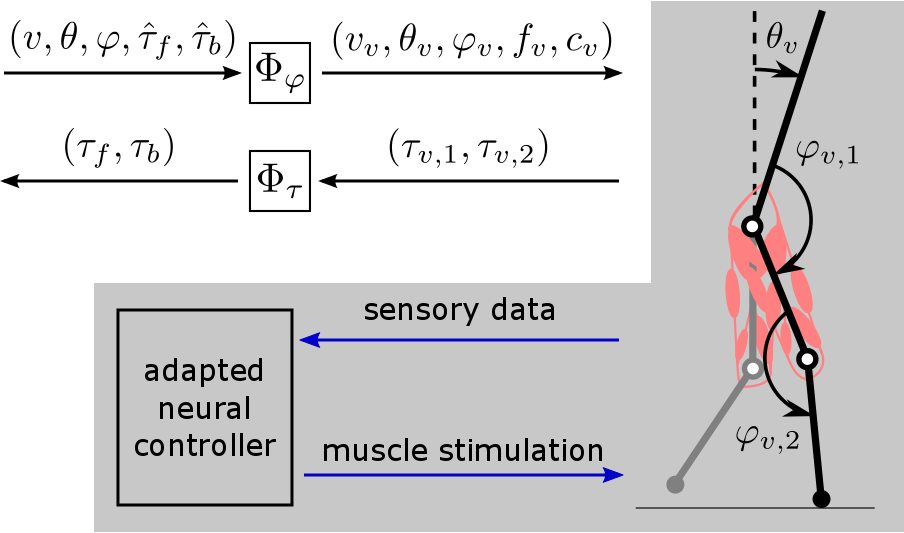
\includegraphics[width=0.6\textwidth]{img/VNMC.png}
\caption{\small{Virtual neuromuscular control.
VNMC maps the robot's state, $(v, \theta, \varphi, \hat{\tau}_f, \hat{\tau}_b)$, to virtual measurements required to emulate a neuromuscular model, $(v_v, \theta_v,  \varphi_v, f_v, c_v)$, where $\varphi$ are joint angles, and $f_v$ and $c_v$ are force and contact data of the virtual leg.
The virtual neuromuscular model (in the gray box) outputs virtual joint torques, $(\tau_{v,1}, \tau_{v,2})$, that are mapped to desired robot joint torques, $(\tau_f, \tau_b)$, which are tracked by the SEA controller.}}
\label{fig:VNMC}
\end{figure}

% P1 - summary
We adapt a previously proposed virtual neuromuscular controller (VNMC) \cite{batts2015toward} adapted for ATRIAS. VNMC maps a neuromuscular model to the robot's topology and emulates it to generate desired motor torques, which is sent to the SEA controller (Figure \ref{fig:VNMC}).
The emulated neuromuscular model, which is originally developed to study human locomotion, consists of primarily spinal reflexes, and with appropriate sets of control parameters, it generates diverse human locomotion behaviors \cite{song2015neural}, such as walk, run,turn, walk up stairs, etc. The VNMC control consists of 6 muscles on each leg - the hip flexors (HFL), the glutei (GLU), the hamstrings (HAM), the rectus femoris (RF), the vastii (VAS) and the biceps femoris (BFSH). Since ATRIAS doesn't have any ankles, these muscles are removed from the model. The feedbacks are similar to the ones described in \ref{sec:NMC}, and details can be found in \cite{song2015neural}.

% P2 - improvements from previous version
For this study, we adapt the previous VNMC \cite{batts2015toward} by removing some unnecessary biological components while preserving its basic functionalities.
First, the new VNMC directly uses joint angular and angular velocity data instead of estimating it from physiologically plausible sensory data, such as muscle fiber states, when applicable.
Second, most of the neural transmission delays are removed, except the ones utilized by the controller.

The adapted VNMC consists of 50 control parameters including feedback gains for each muscle feedback in swing and stance, pre-stimulations for each muscle in swing and stance, high level leg placement gains and desired trunk inclination. When optimized using covariance matrix adaptation evolution strategy \cite{hansen2006cma}, it can control ATRIAS to walk on rough terrains with height changes of $\pm$20 cm in planar simulation. The original VNMC in \cite{batts2015toward} doesn't start from rest, which is impossible to achieve on a robot. To overcome this problem, for now, we start with a 5-dimensional walking controller that can start from rest. Once a desired speed if reached, we switch to the virtual neuromuscular control.

\section{Inaccurate simulations for constructing kernels}

To compare the performance of different methods that can be used to transfer information from simulation to hardware, we create a series of increasingly approximate simulators. These simulators emulate increasing mismatch between simulation and hardware and its effect on the information transfer. Commonly seen discrepancies between simulation and hardware can be classified into three categories: incorrect dynamics parameters, incorrect dynamics models and incorrect environment/task. Incorrect dynamics parameters include discrepancies such as wrong mass, inertia, CoM location of links of the robot. Incorrect models on the other hand are more systematic errors, such as incorrect friction models, actuator dynamics and unmodeled parts of the robot. The third type of discrepancy occurs when simulation is modelling a task different from what is seen on hardware, for example walking on flat ground vs climbing stairs.  We perturb our simulation to create discrepancies of the first two kinds described above, and test the performance of BO at optimizing a 5, 9 and 50 dimensional controller. This allows us to study the effect of increasing mismatch between simulation and hardware on the performance of our proposed approach.

\subsection{Incorrect dynamics parameters}
Our first set of experiments create a  \textit{``simulated hardware"} that is increasingly different from the simulation, in which the DoG features were collected. This is done by changing the mass, inertia, center of mass location of each link of the  by up to $\pm x\%$ ($x = 20, 40, 60$) of its original value. This perturbed simulation now serves as a test hardware for features calculated in the unperturbed simulator. The friction coefficient of the ground contact models, ground stiffness and actuator delay is also changed by the same amount. 
Unlike domain-randomization, from \cite{mordatch2015ensemble}, instead of training on perturbations, we test on these perturbations. This setup is designed to test whether our approach can be used even when the scale of mismatch between simulation and hardware is unknown a-priori.

\subsection{Incorrect dynamics models}
In this setting, the high-fidelity ATRIAS simulator~\citep{martin2015robust}, is the \textit{simulated ``hardware"}. We make dynamics approximations to the original simulator, which are used commonly in simulators to decrease fidelity and increase simulation speed. For example, the complex dynamics of harmonic drives are approximated as a torque multiplication, and the boom is removed from the simulation, leading to a two-dimensional simulator. These approximate simulators now become the \textit{simulated ``simulators"}. As the approximations in these simulators are increased, we expect the performance of methods that utilize simulation for optimization on hardware to deteriorate.

The details of the approximate simulators are described below:

\begin{enumerate}
    \item \textbf{Simulation with simplified gear dynamics} : The ATRIAS robot has geared DC motors attached to leaf springs on the legs. Their high gear ratio of 50 is achieved through a harmonic drive. In the original simulator, this drive is modelled using gear constraints in MATLAB SimScape Multibody simulation environment. These require significant computation time as the constraint equations have to be solved at every time instant, but lead to a very good match between the robot and simulation. We replace this model with a commonly used approximation for geared systems -- multiplying the rotor torque by the gear ratio. This reduces the simulation time to about a third of the original simulator, but leads to an approximate gear dynamics model.

    \item \textbf{Simulation with no boom and simplified gear dynamics} : The ATRIAS robot walks on a boom in our hardware experiments. The boom leads to lateral torques on the robot, which have vertical and horizontal force components that need to be considered in a realistic simulation of the robot. In our second approximation, we remove the boom from the original simulator and constraint the motion of the robot to a 2-dimensional plane, making a truly two-dimensional simulation of ATRIAS. This is a common approximation for two-dimensional robots. Since this approximation has both simplified gear dynamics and no boom, it is further from the original simulator than the first approximation.

\end{enumerate}

\begin{figure}
    \centering
    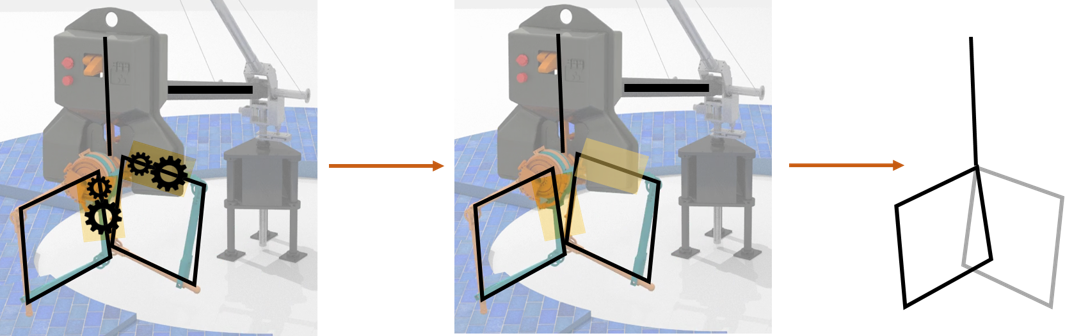
\includegraphics[width = 0.8\textwidth]{img/atrias_gear_boom_simplification.png}
    \caption{Different fidelity simulators for ATRIAS. The original simulator (left) is very high-fidelity with complex gear and boom dynamics. The second simulator (middle) has an approximate gear dynamics model and the third simulator (right) simulates a 2-dimensional robot without boom or gear dynamics.}
    \label{fig:simulators}
\end{figure}

A visual illustration of these approximations is shown in Figure \ref{fig:simulators}. The advantage of such an arrangement is that we can extensively test the effect of un-modelled and wrongly modelled dynamics on information transfer between simulation and hardware. Even in our high-fidelity original simulator, there are several un-modelled components of the actual hardware. For example, the non-rigidness of the robot parts, misaligned motors and relative play between joints. In our experiments, we find that the 50-dimensional VNMC is a sensitive controller, with little hope of directly transferring from simulation to hardware. Anticipating this, we can now test several methods of compensating for this mismatch using our increasingly approximate simulators. In the future, we would like to take this approximations further and study when there is useful information even in over-simplified simulations of legged systems.


